%%%%%%%%%%%%%%%%%%%%%%%%%%%%%%%%%%%%%%%%%%%%%%%%%%%%%%%%%%%%%%%%%%%%%%%%%%%%
% Ausarbeitung
%%%%%%%%%%%%%%%%%%%%%%%%%%%%%%%%%%%%%%%%%%%%%%%%%%%%%%%%%%%%%%%%%%%%%%%%%%%%

% Eine Dokumentation zur TU Darmstadt-LaTeX-Vorlage ist nach der installation in etwa hier zu finden (User_X ersetzen durch den aktuellen Benutzer):
% C:\Users\User_X\AppData\Local\Programs\MiKTeX\doc\latex\tuda-ci

%%%%%%%%%%%%%%%%%%%%%%%%%%%%%%%%%%%%%%%%%%%%%%%%%%%%%%%%%%%%%%%%%%%%%%%%%%%%
% Grundeinstellungen

\documentclass[
	ngerman,
	ruledheaders=section,%Ebene bis zu der die Überschriften mit Linien abgetrennt werden, vgl. DEMO-TUDaPub
	class=report,% Basisdokumentenklasse. Wählt die Korrespondierende KOMA-Script Klasse
	thesis={type=master, instbox=false},% Dokumententyp Thesis, für Dissertationen siehe die Demo-Datei DEMO-TUDaPhd
	accentcolor=9c,% Auswahl der Akzentfarbe
	custommargins=false,% Ränder werden mithilfe von typearea automatisch berechnet
	marginpar=false,% Kopfzeile und Fußzeile erstrecken sich nicht über die Randnotizspalte
	BCOR=5mm,%Bindekorrektur, falls notwendig
	BCORtitlepage=true,
	%parskip=half-,%Absatzkennzeichnung durch Abstand vgl. KOMA-Sript
	fontsize=11pt,%Basisschriftgröße laut Corporate Design ist mit 9pt häufig zu klein
	logofile={figures/00_Formalien/tuda_logo.pdf},%Falls die Logo Dateien nicht vorliegen
	title=small,
	twoside=false
]{tudapub}

%%%%%%%%%%%%%%%%%%%%%%%%%%%%%%%%%%%%%%%%%%%%%%%%%%%%%%%%%%%%%%%%%%%%%%%%%%%%
% Pakete einbinden

\usepackage{fontspec}
\usepackage{caption}


% Sprachanpassung & Verbesserte Trennregeln
\usepackage[english, main=ngerman]{babel}
\usepackage[autostyle]{csquotes}% Anführungszeichen vereinfacht
\usepackage{microtype}
\usepackage{enumitem} %für z.B fettgerduckte Zahlen bei einer Aufzählung

% float options
\usepackage{float}

% Literaturverzeichnis
\usepackage[backend=biber, style=alphabetic]{biblatex}
\addbibresource{bibliography/Literaturverzeichnis.bib} % Literaturliste


% Tabellen
%\usepackage{array}     % Basispaket für Tabellenkonfiguration, wird von den folgenden automatisch geladen
\usepackage{tabularx}   % Tabellen, die sich automatisch der Breite anpassen
\usepackage{longtable} % Mehrseitige Tabellen
%\usepackage{xltabular} % Mehrseitige Tabellen mit anpassarer Breite
\usepackage{booktabs}   % Verbesserte Möglichkeiten für Tabellenlayout über horizontale Linien
\usepackage{multirow}

% Paketvorschläge Mathematik
\usepackage{mathtools} % erweiterte Fassung von amsmath
%\usepackage[]{amsmath}
\usepackage[single]{accents}
%\usepackage{amssymb}   % erweiterter Zeichensatz
%\usepackage{siunitx}   % Einheiten

% Pakete für Grafiken
\usepackage{graphicx}
\graphicspath{{figures/00_Formalien/}{figures/01_Zusammenfassung/}{figures/02_Einleitung/}{figures/03_Grundlagen/}{figures/04_Aktueller Forschungsstand und Forschungsfrage/}{figures/05_Hauptteil/}{figures/06_Vergleich/}{figures/07_Fazit/}{figures/99_Anhang/}} % Standardpfade für Grafikimport, müssen an jeweilige Ordnerstruktur angepasst werden
\usepackage{xcolor}
\usepackage{transparent}
\usepackage{pdfpages}

\usepackage{setspace} % Zeilenabstände

\usepackage{pifont}% Zapf-Dingbats Symbole
\newcommand*{\FeatureTrue}{\ding{52}}
\newcommand*{\FeatureFalse}{\ding{56}}

% Hurenkinder und Schusterjungen verhindern (Das wird wirklich so genannt, hab ich mir nicht ausgedacht xD)
\clubpenalty10000
\widowpenalty10000
\displaywidowpenalty=10000

%Definiert Länge der Einrückung bei neuem Absatz
\setlength{\parindent}{0pt}

%URL font style
\urlstyle{same}

% Zusätzliche Überschriften Ebene
%\setcounter{tocdepth}{4}
\setcounter{secnumdepth}{4}

% Silbentrennung
\hyphenation{Re-luk-tanz-ma-schi-nen}

\captionsetup{font=normal, labelfont={normal}}


\begin{document}

% Metadaten der PDF-Datei
\Metadata{
	title=Energetische Flexibilisierung des Betriebs einer Durchlaufreinigungsanlage durch techno-ökonomische Optimierung auf der Betriebsleitebene,
	author=Jonas Gölz,
	keywords={Synchron-Reluktanzmaschine \sep Rotorgeometrie \sep Drehmomentwelligkeit \sep Serienfertigung \sep Symmetrieeigenschaften}
}


        
%%%%%%%%%%%%%%%%%%%%%%%%%%%%%%%%%%%%%%%%%%%%%%%%%%%%%%%%%%%%%%%%%%%%%%%%%%%%
% Titelseite
\title{\begin{spacing}{2}{\fontsize{23}{23} \selectfont Energetische Flexibilisierung des Betriebs einer Durchlaufreinigungsanlage durch techno-ökonomische Optimierung auf der Betriebsleitebene}\end{spacing}}

\subtitle{Energetic flexibilization of the operation of an Aqueous Parts Cleaning Machine through techno-economic optimization at the Manufacturing Excution System level}
\author[Jonas Gölz]{Jonas Gölz}%optionales Argument ist die Signatur

\reviewer{Prof. Dr.-Ing. Matthias Weigold}%Gutachter

%Diese Felder werden untereinander auf der Titelseite platziert.
%\department ist eine notwendige Angabe, siehe auch dem Abschnitt `Abweichung von den Vorgaben für die Titelseite'
\department{mb} % Das Kürzel wird automatisch ersetzt und als Studienfach gewählt, siehe Liste der Kürzel im Dokument.

\submissiondate{24. Oktober 2024}
%\examdate{4. Februar 2021}
%\date{4. Februar 2021}
\publishers{}
%\titleaddendum{Betreuer(intern): Dipl.-Ing.\newline
%Betreuer(extern): M.Sc. }

%\addTitleBoxLogo*{
\includegraphics[width=0.66\linewidth]{figures/00_Formalien/PTW_Logo_CMYK_whitebackground.pdf}}
\addTitleBoxLogo*{
\includegraphics[width=1.0\linewidth]{figures/00_Formalien/PTW_Logo.pdf}}

\maketitle


%%%%%%%%%%%%%%%%%%%%%%%%%%%%%%%%%%%%%%%%%%%%%%%%%%%%%%%%%%%%%%%%%%%%%%%%%%%%
% Aufgabenstellung
\pagenumbering{gobble} 	% einstellen der Seiten Nummerierung {gobble=keine Seitenzahl, Roman=große römische Zahlen, roman=kleine römische Zahlen, arabic=arabische Zahlen}

%\noindent 	% einrücken des Textes zu beginn eines neuen Absatzes unterdrücken (hier benutzt, damit die folgende Grafik nicht verschoben wird)
%\includegraphics[scale=0.95]{Texte/Aufgabenstellung.eps} 	% einbinden einer Abbildung [Skalierung]{Dateipfad ausgehend vom Ablageort der Hauptdatei/Dateiname mit Dateiendung z.B. eps, png, ...}
\newpage
 %$\quad$
\includepdf[pages=-]{figures/00_Formalien/Aufgabenstellung.pdf}

\newpage
%%%%%%%%%%%%%%%%%%%%%%%%%%%%%%%%%%%%%%%%%%%%%%%%%%%%%%%%%%%%%%%%%%%%%%%%%%%%
% Eigenständigkeitserklärung

% Version der Erklärung aus tuda-ci-package
\affidavit[signature=Jonas Gölz,signature-image={
\includegraphics[width=\width]{figures/00_Formalien/Signatur_MaxMustermann.png}}]


\newpage
% Leere Seite
%\quad
%\newpage

%%%%%%%%%%%%%%%%%%%%%%%%%%%%%%%%%%%%%%%%%%%%%%%%%%%%%%%%%%%%%%%%%%%%%%%%%%%%
% Römische Seitenzahlen
\pagenumbering{Roman}
%\frontmatter

%%%%%%%%%%%%%%%%%%%%%%%%%%%%%%%%%%%%%%%%%%%%%%%%%%%%%%%%%%%%%%%%%%%%%%%%%%%%
% Abstract/Zusammenfassung
\pdfbookmark[0]{Abstract}{abstract}	% Lesezeichen im PDF Reader [Gliederungstiefe (Position in Lesezeichenbaum) -1, 0, ...,5]{Titel des Lesezeichens}{label auf das verwiesen wird also die Stelle in Textdokument zu der hingesprungen werden soll}
\section*{Zusammenfassung}
\vspace*{0.2cm} 
\textbf{Thema: Titel der Arbeit}\\
\\
Text text text text text text text text text text text text text text text text text text text text text text text text text text text text text text text text text text text text text text text text text text text text text text text text text text text text text text text text text text text text text text text text text text text text text text text text text\\
\\\textbf{Schlüsselwörter:} Synchron-Reluktanzmaschine, Rotorblechschnitt, Rotorgeometrie, Drehmomentwelligkeit, Serienfertigung, Symmetrieeigenschaften

\phantomsection

%%%%%%%%%%%%%%%%%%%%%%%%%%%%%%%%%%%%%%%%%%%%%%%%%%%%%%%%%%%%%%%%%%%%%%%%%%%%
% Inhaltsangabe
\newpage
\makeatletter
\renewcommand*{\@pnumwidth}{3em} % Breite der Box für Seitenzahlen im Inhaltsverzeichnis erhöhen
\makeatother

\pdfbookmark[0]{Inhaltsverzeichnis}{toc}
\tableofcontents % Inhaltsverzeichnis erstellen
% Abstände für Seitenzahlen im Inhaltsverzeichnis erhöhen
\phantomsection

%%%%%%%%%%%%%%%%%%%%%%%%%%%%%%%%%%%%%%%%%%%%%%%%%%%%%%%%%%%%%%%%%%%%%%%%%%%%
% Formelzeichen und Abkürzungen
\newpage
\addcontentsline{toc}{chapter}{Abkürzungsverzeichnis}
%\vspace*{0.025cm}
\chapter*{Abkürzungsverzeichnis}
\begin{spacing}{1.5}
\setlength\LTleft{15pt}
\setlength\LTright{\fill}
\begin{longtable}{ll}
    \textbf{Abkürzung}				&\textbf{Bedeutung}	\\\midrule\endhead
    APCMs							&Aqueous Parts Cleaning Machine\\
    BKV								&Bilanzkreisverantwortliche\\
    CAD								&Computer-Aided Design\\
    CS								&Companion Specifications\\
   	DLRA							&Durchlaufreinigungsanlage\\
   	DR								&Demand Response\\
   	DSM								&Demand-side management\\
   	EEG								&Erneuerbare-Energien-Gesetz\\
    EEX								&European Energy Exchange\\
    ERP								&Enterprise Resource Planning\\
    HTTPS							&Hypertext Transfer Protocol Secure\\
    JSON							&JavaScript Object Notation\\
    KWKG							&Kraft-Wärme-Kopplungsgesetz\\
    MES								&Manufacturing Execution Systems\\
    MSB								&Messstellenbetreiber\\
    OPC UA							&OPC Unified Architecture\\
    OPC UA FX						&OPC UA Field eXchange\\
    OTC								&Over-the-Counter\\
    PXE								&Power Exchange Central Europe\\
    SDKs							&Software Development Kits\\
    StromNEV						&Stromnetzentgeltverordnung\\
	SynRM							&Synchron-Reluktanzmaschine\\
	ÜNB								&Übertragungsnetzbetreiber\\
	VNB								&Verteilnetzbetreiber\\
	XML								&Extensible Markup Language\\

  \end{longtable}
\end{spacing}

                    
%\newpage
\phantomsection
\addcontentsline{toc}{chapter}{Formelzeichen}
%\vspace*{0.025cm}
\chapter*{Formelzeichen}
\section*{Allgemeine Hinweise}
%
%\begin{spacing}{1.5}
%	\setlength\LTleft{100pt}
%	\setlength\LTright{\fill}
%	%\begin{longtable}{@{\extracolsep{\fill}}cl}
%	\begin{longtable}{cl}
%		$\dot{X}$				&zeitliche Ableitung\\
%		$\hat{X}$				&Amplitudenwert \\
%		$\vec{X}$				&Vektor \\
%		$\underline{X}$			&Komplexer Phasor\\
%		$\underline{X}^*$ 		&Konjugiert-Komplexer Phasor\\
%		$\textbf{X}$			&Matrix\\
%	\end{longtable}
%\end{spacing}
%%
%\section*{Indizes}
%%
%Treten mehrere der hier aufgelisteten Indizes auf, so werden diese mit Komma getrennt angeschrieben.
%\begin{spacing}{1.5}
%	\setlength\LTleft{100pt}
%	\setlength\LTright{\fill}
%	%\begin{longtable}{@{\extracolsep{\fill}}cl}
%	\begin{longtable}{cl}
%		\textsf{A}				&Pol A\\
%		\textsf{B}				&Pol B\\
%		\textsf{B}				&Gleichungssystem magn. Flussdichte (nur in Kapitel \ref{ch_04MagPotRot})\\
%		\textsf{d}				&$d$-Achse/Komponente\\
%		\textsf{Fe}				&Eisen(-blech)\\
%		\textsf{fb}				&Flusssperre (flux-barrier)\\
%		\textsf{fbe}			&Flusssperrenende (flux-barrier end)\\
%		\textsf{fc}				&Flussleitpfad (flux-carrier)\\
%		\textsf{H}				&Gleichungssystem magn. Feldstärke (nur in Kapitel \ref{ch_04MagPotRot})\\
%		$i$						&Nummer der Flusssperre gezählt von außen nach innen: 1,2,...,$N_\textsf{fb}$\\
%		$j$						&Nummer des Abschnitts für Unterteilung des Flusssperrenendes: 1,2,...\\
%		\textsf{q}				&$q$-Achse/Komponente\\
%		\textsf{R}				&Rotor\\
%		\textsf{S}				&Stator\\
%		\textsf{U}				&Strang U\\
%		\textsf{V}				&Strang V\\
%		\textsf{W}				&Strang W\\
%		\textsf{\delta}			&Luftspalt\\
%		\textsf{\nu}			&Ordnungszahlen der Grund- und Oberwellen im Luftpalt\\
%		\textsf{\xi}			&Ordnungszahlen der Grund- und Oberwellen im Luftpalt\\
%	\end{longtable}
%\end{spacing}
%%
%%
%\section*{Lateinische Formelzeichen}
%\begin{spacing}{1.5}
%	\setlength\LTleft{8pt}
%	\setlength\LTright{\fill}
%	\begin{longtable}{@{\extracolsep{\fill}}ccl}
%		\textbf{Symbol}		&\textbf{Einheit}			&\textbf{Beschreibung}                                           \\\midrule\endhead
%		$A$ 				&$\textsf{m}^{2}$	&Fläche\\
%		$A_{j}$ 		&$\textsf{m}^{2}$	&Querschnittsfläche an der $j$-ten Stützstelle des Flusssperrenendes\\
%		$A_\textsf{S}$ 		&$\frac{\textsf{A}}{\textsf{m}}$	&Strombelag\\
%		$\tilde{A}_\textsf{S}$&$\frac{\textsf{A}}{\textsf{m}}$	&äquivalenter Strombelag\\
%		$A_\textsf{z}$ 		&$\frac{\textsf{V\cdot s}}{\textsf{m}}$	&Komponente des magn. Vektorpotentials normal zur Blechebene \\
%		$a$ 				&$\textsf{-}$	&Anzahl paralleler Zweige\\
%		$a$ 				&$\frac{\textsf{m}}{\textsf{s}^\textsf{2}}$	&Beschleunigung\\
%		$a_\eta$, $a_\zeta$ &$\frac{\textsf{m}}{\textsf{s}^\textsf{2}}$	&Beschleunigung in Richtung $\eta$, in Richtung $\zeta$\\
%		$B$ 				&$\textsf{T}$	&magnetische Flussdichte\\
%		$B_{j\textsf{a}}$, $B_{j\textsf{b}}$ 		&$\textsf{T}$	&magn. Flussdichte an der $j$-ten Stützstelle $\textsf{a}$,$\textsf{b}$ des Flusssperrenendes\\
%		$B_\textsf{n}$ 		&$\textsf{T}$	&magnetische Flussdichte in Normalenrichtung\\
%		$B_\textsf{t}$ 		&$\textsf{T}$	&magnetische Flussdichte in Tangentenrichtung\\
%		$B_\delta$ 			&$\textsf{T}$	&magnetische Luftspaltflussdichte\\
%		$b_\textsf{Q}$ 		&$\textsf{m}$	&Nutschlitzbreite\\
%		$b_\textsf{0}$ 		&$\textsf{rad}$	&äquivalente Nutschlitzbreite im Bogenmaß (mech.)\\
%		$d_\textsf{A}$ 		&$\textsf{m}$	&Außendurchmesser\\
%		$d_\textsf{Sh}$ 	&$\textsf{m}$	&Wellendurchmesser\\
%		$d_\textsf{Si}$ 	&$\textsf{m}$	&Statorbohrungsdurchmesser\\
%		$E$ 				&$\frac{\textsf{N}}{\textsf{m}^\textsf{2}}$		&Elastizitätsmodul\\
%		$F_{\textsf{L}\eta}$, $F_{\textsf{L}\zeta}$&$\textsf{N}$&Kraft auf das linke Lager in Richtung $\eta$, in Richtung $\zeta$\\
%		$F_{\textsf{R}\eta}$, $F_{\textsf{R}\zeta}$&$\textsf{N}$&Kraft auf das rechte Lager in Richtung $\eta$, in Richtung $\zeta$\\
%		$f_\textsf{t}$ 		&$\frac{\textsf{N}}{\textsf{m}^\textsf{2}}$	&\textit{Maxwell}'sche Schubspannung\\
%		$H$ 				&$\frac{\textsf{A}}{\textsf{m}}$	&magnetische Feldstärke\\
%		$H_{j\textsf{a}}$, $H_{j\textsf{b}}$ 		&$\frac{\textsf{A}}{\textsf{m}}$	&magn. Feldstärke an der $j$-ten Stützstelle $\textsf{a}$,$\textsf{b}$ des Flusssperrenendes\\
%		$H_\textsf{t}$ 		&$\frac{\textsf{A}}{\textsf{m}}$	&magnetische Feldstärke in Tangentenrichtung\\
%		$H_\delta$ 			&$\frac{\textsf{A}}{\textsf{m}}$	&magnetische Feldstärke im Luftspalt\\
%		$I_\textsf{S}$		&$\textsf{A}$	&Strangstrom Effektivwert\\
%		$i_\textsf{S}$ 		&$\textsf{A}$	&Strangstrom Augenblickswert\\
%		$i_\textsf{C}$ 		&$\textsf{A}$	&Spulenstrom Augenblickswert\\
%		$j$ 				&$\textsf{-}$	&imaginäre Einheit\\
%		$J_{\textsf{H,fc,}i}$, $J_{\textsf{M,fc,}i}$, $J_{\textsf{L,fc,}i}$&$\textsf{-}$	&Integrale für Berechnung der magn. Potentiale der Flussleitpfade\\
%		$K_\delta$			&$\frac{\textsf{V\cdot s}}{\textsf{A}}$				&Konstante für Berechnung der magn. Potentiale der Flussleitpfade\\
%		$k_\textsf{C}$ 			&$\textsf{-}$	&\textit{Carter}-Faktor\\
%		$k_{\textsf{d,}\nu}$&$\textsf{-}$	&Zonenfaktor\\
%		$K_{h\textsf{,}i}$	&$\textsf{-}$	&Proportionalitätsfaktor der $h$-ten Drehmomentharmonischen\\
%		 & &für die $i$-te Flusssperre bei Rotorvariante 1\\
%		$K_{h\textsf{,}i\textsf{,AB}}$	&$\textsf{-}$	&Proportionalitätsfaktor der $h$-ten Drehmomentharmonischen\\
%		 & &für die $i$-te Flusssperre in Pol \textsf{A} und \textsf{B} bei Rotorvariante 2\\
%		$k_{\textsf{p,}\nu}$&$\textsf{-}$	&Sehnungsfaktor\\
%		$k_\textsf{Q}$		&$\textsf{-}$	&Verhältnis Statornutbreite zu Nutteilung\\
%		$k_{\textsf{w,}\nu}$&$\textsf{-}$	&Wicklungsfaktor\\
%		$k_\textsf{w,fc}$	&$\textsf{-}$	&Skalierungsfaktor Flussleitpfadbreite an der $q$-Achse\\
%		$k_\textsf{w,q}$	&$\textsf{-}$	&Verhältnis von Eisen zu Luft in der $q$-Achse\\
%		$k_\textsf{Y}$		&$\textsf{-}$	&Verhältnis Nuttiefe zu Differenz Statoraußen- zu Statorinnenradius\\
%		$L$					&$\textsf{H}$	&Selbsinduktivität\\
%		$l_{\textsf{fb,}i}$ 	&$\textsf{m}$	&Länge der $i$-ten Flusssperre\\
%		$l_\textsf{Fe}$ 	&$\textsf{m}$	&Aktivlänge\\
%		$l_\textsf{Q}$ 		&$\textsf{m}$	&Statornuttiefe\\
%		$l_\textsf{R}$ 		&$\textsf{m}$	&Länge des Rotors\\
%		$M_\textsf{e}$		&$\textsf{Nm}$	&elektromagnetisches Drehmoment\\
%		$M_\textsf{e,max}$	&$\textsf{Nm}$	&maximales Drehmoment\\
%		$M_\textsf{e,mean}$	&$\textsf{Nm}$	&Mittelwert des elektromagnetischen Drehmoments\\
%		$M_{h}$		&$\textsf{Nm}$	&elektromagnetisches Drehmoment der $h$-ten Harmonischen\\
%		$m$					&$\textsf{-}$	&Strangzahl\\
%		$m$					&$\textsf{kg}$	&Masse\\
%		$m_\textsf{R}$		&$\textsf{kg}$	&Rotormasse\\
%		$N$ 				&$\textsf{-}$	&magnetisch wirksame Strangwindungszahl\\
%		$N_\textsf{fb}$ 	&$\textsf{-}$	&Anzahl Flusssperren pro Pol\\
%		$N_\textsf{C}$ 		&$\textsf{-}$	&Spulenwindungszahl\\
%		$P_\textsf{e}$ 		&$\textsf{W}$	&elektrische Wirkleistung\\
%		$P_\textsf{m}$ 		&$\textsf{W}$	&mechanische Leistung\\
%		$p$					&$\textsf{-}$	&Polpaarzahl\\
%		$p_\textsf{F,A}$ 	&$\frac{\textsf{N}}{\textsf{m}^\textsf{2}}$		&Fugendruck\\
%		$p_\textsf{F,PA}$ 	&$\frac{\textsf{N}}{\textsf{m}^\textsf{2}}$		&Fugendruck bei vollständiger Plastifizierung des Außenteils\\
%		$p_\textsf{min}$ 	&$\frac{\textsf{N}}{\textsf{m}^\textsf{2}}$		&Mindestfugendruck\\
%		$Q$ 				&$\textsf{-}$	&Statornutzahl\\
%		$Q_\textsf{A}$ 		&$\textsf{-}$	&Durchmesserverhältnis\\
%		$q$					&$\textsf{-}$	&Spulen pro Pol und Strang\\
%		$R_\textsf{m}$ 		&$\frac{\textsf{N}}{\textsf{m}^\textsf{2}}$		&Zugfestigkeit\\
%		$R_\textsf{m}$ 		&$\frac{\textsf{A}}{\textsf{V\cdot s}}$	&magnetischer Widerstand\\
%		$R_{\textsf{m,fb,}i}$ &$\frac{\textsf{A}}{\textsf{V\cdot s}}$	&magnetischer Widerstand der $i$-ten Flusssperre\\
%		$R_{\textsf{m,fbe,}i\textsf{,n}}$&$\frac{\textsf{A}}{\textsf{V\cdot s}}$	&magnetischer Ersatzwiderstand für das $i$-te Flusssperrenende\\
%		 & &in negativer Drehrichtung von $\vartheta$\\
%		$R_{\textsf{m,fbe,}i\textsf{,p}}$&$\frac{\textsf{A}}{\textsf{V\cdot s}}$	&magnetischer Ersatzwiderstand für das $i$-te Flusssperrenende\\
%		 & &in positiver Drehrichtung von $\vartheta$\\
%		$R_\textsf{p0.2}$ 	&$\frac{\textsf{N}}{\textsf{m}^\textsf{2}}$		&0.2\,\% Dehngrenze/Streckgrenze\\
%		$R_\textsf{S}$ 		&$\Omega$		&elektrischer Strangwiderstand\\
%		$r$ 				&$\textsf{m}$	&Radius\\
%		$r_\textsf{A}$ 		&$\textsf{m}$	&Radius außen\\
%		$r_\textsf{I}$ 		&$\textsf{m}$	&Radius innen\\
%		$r_\textsf{Si}$ 	&$\textsf{m}$	&Innenradius des Statorblechs\\
%		$r_\textsf{Sh}$ 	&$\textsf{m}$	&Außenradius der Welle im Bereich des Rotorblechpakets\\
%		$r_\textsf{So}$ 	&$\textsf{m}$	&Außenradius des Statorblechs\\
%		$r_\textsf{Ri}$ 	&$\textsf{m}$	&Innenradius des Rotorblechs\\
%		$r_\textsf{Ro}$ 	&$\textsf{m}$	&Außenradius des Rotorblechs\\
%		$\text{r}_{\textsf{fb,}\eta\textsf{,}i}$&$\textsf{-}$&Winkelverhältnis Platzierung der Steuerungspunkte an den\\
%		 & &Flusssperrenenden\\
%		$\text{r}_\textsf{mid}$&$\textsf{-}$&Längenverhältnis Platzierung der Steuerungspunkte im Mittelbereich\\
%		 & &des Flussleitpfads\\
%		$\text{r}_\textsf{q}$&$\textsf{-}$&Längenverhältnis Platzierung der Steuerungspunkte an der $q$-Achse\\
%		$S_\textsf{PA}$ 	&$\textsf{-}$	&Sicherheit gegen vollständige Plastifizierung des Außenteils\\
%		$S_\textsf{R}$ 		&$\textsf{-}$	&Sicherheit gegen Durchrutschen der Welle\\
%		$s$ 				&$\textsf{m}$	&Weg\\
%		$s_\textsf{Q}$ 		&$\textsf{m}$	&Weg einer Feldlinie im Nutöffnungsbereich\\
%		$s_\textsf{Z}$ 		&$\textsf{m}$	&Weg einer Feldlinie im Zahnbereich\\
%		$U$ 				&$\textsf{V}$	&elektrische Spannung\\
%		$U_\textsf{ind}$ 	&$\textsf{V}$	&induzierte Spannung\\
%		$U_\textsf{max}$ 	&$\textsf{m}$	&maximales Übermaß\\
%		$U_\textsf{min}$ 	&$\textsf{m}$	&minimales Übermaß\\
%		$U_\textsf{S}$ 		&$\textsf{V}$	&Strangspannung\\
%		$u$ 				&$\textsf{m}$	&Verschiebung\\
%		$V$					&$\textsf{A}$	&magnetische Spannung/Potential\\
%		$V_\textsf{C}$		&$\textsf{A}$	&magnetische Spannung im Luftspalt für eine Spule\\
%		$V_\textsf{Gr}$		&$\textsf{A}$	&magnetische Spannung im Luftspalt für eine Spulengruppe\\
%		$V_\textsf{R,High}$, $V_\textsf{R,Low}$&$\textsf{A}$	&Randbedingungen für das magn. Potential am Flusssperrenende\\
%		$V_\textsf{Strang}$	&$\textsf{A}$	&magnetische Spannung im Luftspalt für einen Strang\\
%		$V_\delta$			&$\textsf{A}$	&magnetische Spannung im Luftspalt\\
%		$V_{\delta\textsf{,1}}$	&$\textsf{A}$	&magnetische Spannung der Grundwelle\\
%		$W$ 				&$\textsf{-}$	&Spulenweite\\
%		$w_{\textsf{fb,}i}$ 	&$\textsf{m}$	&Breite der $i$-ten Flusssperre\\
%		$w_{\textsf{fbe,}i}$ 	&$\textsf{m}$	&Breite des $i$-ten Flusssperrenendes\\
%		$w_{\textsf{fc,}i}$ 	&$\textsf{m}$	&Breite des $i$-ten Flussleitpfads\\
%		$X$ 				&$\Omega$		&Reaktanz\\
%		$x$ 				&$\textsf{m}$	&(Umfangs-)Koordinate\\
%		$x$, $y$, $z$		&$\textsf{m}$	&statorfeste Koordinaten\\
%		$x$, $\eta$, $\zeta$	&$\textsf{m}$		&rotorfeste Koordinaten\\
%	\end{longtable}
%\end{spacing}
%%
%%
%\newpage
%\section*{Griechische Formelzeichen}
%\begin{spacing}{1.5}
%	\setlength\LTleft{8pt}
%	\setlength\LTright{\fill}
%	\begin{longtable}{@{\extracolsep{\fill}}ccl}
%		\textbf{Symbol}			&\textbf{Einheit}			&\textbf{Beschreibung}                                           \\\midrule\endhead
%		$\alpha_\textsf{fb}$	&$\textsf{rad}$		&Winkel der Flusssperrenbreite an den Enden\\
%		$\alpha_\textsf{k}$		&$\textsf{-}$		&Kerbformzahl\\
%		$\beta$					&$\textsf{rad}$		&Statorstromwinkel (el.)\\
%		$\gamma$				&$\textsf{rad}$		&Umfangswinkel (el.)\\
%		$\gamma_\textsf{m}$		&$\textsf{rad}$				&Rotorpositionswinkel (mech.)\\
%		$\gamma_\textsf{R}$		&$\textsf{rad}$			&rotorfester Umfangswinkel von der $d$-Achse aus (mech.)\\
%		$\gamma_\textsf{S}$		&$\textsf{rad}$			&statorfester Umfangswinkel (mech.)\\
%		$\Delta l_\textsf{q}$ 	&$\textsf{m}$		&Abstand zur $q$-Achse für die Ermittlung der Funktion $f_\textsf{q,fc}(\vartheta)$\\
%		$\Delta M_\textsf{e,rel}$&$\textsf{-}$		&relative Drehmomentwelligkeit\\
%		$\Delta r_\textsf{1}$, $\Delta r_\textsf{2}$&$\textsf{m}$		&Radiusdifferenzen für die Ermittlung der Funktion $f_\textsf{mid,fc}(\vartheta)$\\
%		$\Delta s$ 				&$\textsf{m}$		&Abstand zur Sekante für die Ermittlung der Funktion $f_\textsf{mid,fc}(\vartheta)$\\
%		$\Delta s_\textsf{q}$ 	&$\textsf{m}$		&Abstand zur Normalen auf die $q$-Achse für die Ermittlung der Funktion $f_\textsf{q,fc}(\vartheta)$\\
%		$\Delta V$				&$\textsf{A}$		&Differenz zweier magnetischer Potentiale\\
%		$\Delta \vartheta_{\textsf{fb,}i}$&$\textsf{rad}$&Winkeldifferenz der $i$-ten Flusssperre zwischen Pol $\textsf{A}$ und Pol $\textsf{B}$ \\
%		$\delta$				&$\textsf{m}$		&Luftspaltweite\\
%		$\varepsilon_\textsf{r}$&$\textsf{-}$		&radiale Dehnung\\
%		$\varepsilon_\textsf{t}$&$\textsf{-}$		&tangentiale Dehnung\\
%		$\zeta_\textsf{A}$    	&$\textsf{-}$		&bezogener Plastizitätsdurchmesser\\
%		$\eta_\nu$, $\eta_\xi$	&$\textsf{rad}$		&Ordnungszahlen abhängiger Winkel analytische Drehmomentberechnung\\
%		$\Theta$				&$\textsf{A}$		&Durchflutung\\
%		$\Theta_\textsf{C}$		&$\textsf{A}$		&Spulendurchflutung\\
%		$\Theta_\textsf{Q}$		&$\textsf{A}$		&Nutdurchflutung\\
%		$\Theta_{\textsf{x}\eta}$, $\Theta_{\textsf{x}\zeta}$&$\textsf{kg}\cdot \textsf{m}^\textsf{2}$		&Massendeviationsmomente\\
%		$\vartheta$				&$\textsf{rad}$		&rotorfester Umfangswinkel von der $q$-Achse aus (mech.)\\
%		$\vartheta_{\textsf{fb,}i}$				&$\textsf{rad}$		&Positionswinkel der $i$-ten Flusssperre (mech.)\\
%		$\kappa$				&$\textsf{-}$	&Krümmung\\
%		$\kappa_\textsf{L}$		&$\textsf{-}$	&Verhältnis der Induktivitäten der $d$- und $q$-Achse\\
%		$\lambda$				&$\frac{\textsf{V\cdot s}}{\textsf{A} \cdot \textsf{m}^\textsf{2}}$	&flächenbezogener magnetischer Leitwert\\
%		$\lambda_{\textsf{fb,}j}$ &$\frac{\textsf{V\cdot s}}{\textsf{A}}$		&Leitwert des $j$-ten Teilstücks am Flusssperrenende\\
%		$\lambda_\delta$		&$\frac{\textsf{V\cdot s}}{\textsf{A} \cdot \textsf{m}^\textsf{2}}$		&flächenbezogener magnetischer Leitwert des Luftspalts\\
%		$\lambda_{\delta\textsf{,}j}$&$\frac{\textsf{V\cdot s}}{\textsf{A}}$  &Leitwert des $j$-ten Luftspaltteilstücks\\
%		$\tilde{\lambda}$		&$\textsf{-}$		&dimensionsloser Leitwert des Luftspalts\\
%		$\mu$					&$\textsf{-}$		&relative Permeabilität\\
%		$\mu$					&$\textsf{-}$		&Querkontraktionszahl\\
%		$\mu_\textsf{H}$		&$\textsf{-}$		&Haftreibungskoeffizient\\
%		$\mu_0$					&$\frac{\textsf{V\cdot s}}{\textsf{A\cdot m}}$		&magnetische Feldkonstante\\
%		$\nu$					&$\textsf{-}$		&Ordnungszahl magnetisches Potential/Strombelag\\
%		$\nu_\textsf{S}$		&$\textsf{-}$		&Ordnungszahl Nutöffnungseinfluss\\
%		$\xi$    				&$\textsf{-}$		&Ordnungszahl magnetisches Potential/Strombelag\\
%		$\xi_\textsf{W,max}$    &$\textsf{-}$		&bezogenes Höchstübermaß\\
%		$\rho$					&$\frac{\textsf{kg}}{\textsf{m}^\textsf{3}}$			&Dichte\\
%		$\rho_{i\textsf{,}\nu}$	&$\textsf{-}$			&dimensionslose Geometriefaktoren für analytische Drehmomentberechnung\\
%		$\sigma_\textsf{r}$		&$\frac{N}{\textsf{m}^\textsf{2}}$	&Radialspannung (mech.)\\
%		$\sigma_\textsf{r,A}$		&$\frac{N}{\textsf{m}^\textsf{2}}$	&Radialspannung am Außenradius (mech.)\\
%		$\sigma_\textsf{r,I}$		&$\frac{N}{\textsf{m}^\textsf{2}}$	&Radialspannung am Innenradius (mech.)\\
%		$\sigma_\textsf{t}$		&$\frac{N}{\textsf{m}^\textsf{2}}$	&Tangentialspannung (mech.)\\
%		$\tau_\textsf{p}$		&$\textsf{m}$		&Polteilung\\
%		$\tau_\textsf{Q}$		&$\textsf{m}$		&Nutteilung\\		
%		$\Phi$					&$\textsf{Wb}$		&magnetischer Fluss\\
%		$\Phi_{\textsf{fb,}i}$	&$\textsf{Wb}$		&magnetischer Fluss über die $i$-te Flusssperre\\
%		$\Phi_{\textsf{S,fc,}i}$	&$\textsf{Wb}$		&magnetischer Fluss vom Stator in den $i$-ten Flussleitpfad für $V_\textsf{R}=0$\\
%		$\varphi_\textsf{S}$	&$\textsf{rad}$		&Phasenwinkel zwischen Strangspannung und Strangstrom\\
%		$\chi_{\textsf{fbe,}i\textsf{,n}}$    	&$\textsf{-}$	&Formfunktion für das magnetische Potential über den Enden der Flusssperren\\
%		 & &in negativer Drehrichtung von $\vartheta$\\
%		$\chi_{\textsf{fbe,}i\textsf{,p}}$    	&$\textsf{-}$	&Formfunktion für das magnetische Potential über den Enden der Flusssperren\\
%		 & &in positiver Drehrichtung von $\vartheta$\\
%		$\Psi$					&$\textsf{V\cdot s}$&Flussverkettung\\
%		$\Psi_\textsf{S}$		&$\textsf{V\cdot s}$&Strangflussverkettung\\
%		$\omega_\textsf{m}$		&$\frac{1}{\textsf{s}}$	&Winkelgeschwindigkeit (mech.)\\
%		$\omega_\textsf{S}$		&$\frac{1}{\textsf{s}}$	&Statorkreisfrequenz (el.)\\
%	\end{longtable}
%\end{spacing}
%                    
\phantomsection
\setcounter{table}{0} % Setzt den Tabellenzähler zurück auf Null, damit die vorherigen Tabellen für die Formelzeichen und Abkürzungen nicht mitgezählt werden

%%%%%%%%%%%%%%%%%%%%%%%%%%%%%%%%%%%%%%%%%%%%%%%%%%%%%%%%%%%%%%%%%%%%%%%%%%%%
% Liste der Abbildungen
\newpage
\addcontentsline{toc}{chapter}{\listfigurename} % zusätzlichen Eintrag zu Verzeichnis hinzufügen, da für das Abbildungverzeichnis/Tabellenverzeichnis nicht automatisch ein Eintrag generiert wird {Wo der Eintrag erfolgen soll, hier toc (Table of contents) im Inhaltsverzeichnis}{Ebene also Kapitel, Unterkapitel, ...}{Bezeichnung Eintrag}
\listoffigures 	% Liste der Abbildung erstellen
\phantomsection

%%%%%%%%%%%%%%%%%%%%%%%%%%%%%%%%%%%%%%%%%%%%%%%%%%%%%%%%%%%%%%%%%%%%%%%%%%%%
% Liste der Tabellen
\newpage
\addcontentsline{toc}{chapter}{\listtablename}
\listoftables % Liste der Tabellen erstellen
\phantomsection

% Leere Seite
\newpage 
\quad 
\newpage

%%%%%%%%%%%%%%%%%%%%%%%%%%%%%%%%%%%%%%%%%%%%%%%%%%%%%%%%%%%%%%%%%%%%%%%%%%%%
% Umstellung von römischen Seitenzahlen auf arabische und speichern der römischen Seitenzahl
\newpage
\newcounter{savecounter} 	% initialisiert einen Zähler der einen Wert speichern kann mit dem Wert Null {Bezeichnung des Zählers}
\setcounter{savecounter}{\value{page}} 	% weist einem Zähler einen Wert zu {Bezeichnung des Zählers}{Wert der zugewiesen werden soll}
\pagenumbering{arabic}
%\mainmatter

%%%%%%%%%%%%%%%%%%%%%%%%%%%%%%%%%%%%%%%%%%%%%%%%%%%%%%%%%%%%%%%%%%%%%%%%%%%%
% Einleitung
\input{texts/02_Einleitung/02_Einleitung.tex}

%%%%%%%%%%%%%%%%%%%%%%%%%%%%%%%%%%%%%%%%%%%%%%%%%%%%%%%%%%%%%%%%%%%%%%%%%%%%
% Grundlagen
\chapter{Grundlagen}
\label{ch_03Grund}
In diesem Abschnitt werden die Grundlagen erläutert, welche den Ausführungen in dieser Arbeit zugrunde liegen. 

\section{Grundlagen1}
Es kann auf andere Kapitel, Gleichungen, Tabellen und Abbildungen verwiesen werden über Labels. Hier Beispiele: Kapitel \ref{ch_03Grundlagen1_1}, Gleichung (\ref{equ_03Grundlagen1_1_1_2}),
Tabelle \ref{tab_03Grundlagen1_1_1},
Abbildung \ref{fig_03Fourier1}

Es ist Sinnvoll auf die Abbildungen und Tabellen immer mit Hilfe dieser Labels zu verweisen, da die Position dieser im Text von TeX so bestimmt wird, dass sich ein gleichmäßiges Schriftbild ergibt. Hierdurch kommen die Abbildungen und Tabellen nicht immer an der Stelle zum liegen an der sie im Code eingefügt sind.

Die Vergebenen Labels müssen immer eindeutig sein. Die Nummerierung bei den Labels wird von TeX immer automatisch beim kompilieren aktualisiert. Ist ein Label nicht Vorhanden beispielsweise aufgrund eines Schreibfehlers, werden an der entsprechenden Stelle Fragezeichen eingefügt, wie hier \ref{Fantasielabel}. Deshalb kann es Sinnvoll sein Stellen an denen noch etwas zu bearbeiten ist mit Fragezeichen zu kennzeichnen und am Ende das Dokument über die Suchfunktion nach Fragezeichen zu durchsuchen, um nichts zu vergessen und Fehler in den Labels zu entdecken.

Bei den Quellenverweisen wird in ähnlicher Form mit Labels gearbeitet. Die Daten zu den Literaturquellen sind in der bib-Datei im bibliography-Ordner hinterlegt. In dieser Datei sind für die Literatur-Einträge auch Labels hinterlegt, welche hier z.B. \cite{Binder.2017} oder optional mit Angabe der Seitenzahl \cite[S.666]{Binder.2017} oder als Aufzählung \cite{Bianchi.2009, Kerdsup.2014, Sanada.2003, Howard.2015} aufgerufen werden können. Die bib-Datei kann entweder händisch erstellt werden (nicht zu empfehlen) oder z.B. über ein Literaturverwaltungsprogramm wie Citavi. Die Labels(bibtex-keys) können in Citavi verändert werden und werden dann beim nächsten Export der bib-Datei eingetragen.


\subsection{Grundlagen1\_1}
\label{ch_03Grundlagen1_1}
Beispiel für eine Aufzählung:

Bei den vereinfachenden Annahmen handelt es sich um die Folgenden \cite{Binder.2017}:
\begin{itemize}
\item Das Eisen wird als näherungsweise unendlich magnetisch leitfähig (ideales Eisen) angenommen $\mu_{\textsf{Fe}} \to \infty$.
\item Das Luftspaltfeld besitzt nur eine radiale Komponente, da die Luftspaltweite $\delta$ viel kleiner ist als die Polteilung $\tau_{\textsf{P}}$. 
\item Es wird ein ebenes zweidimensionales Feld vorausgesetzt; Randeffekte an den Enden der Maschine werden vernachlässigt.
\item Die Spulen und die Nuten, in denen diese liegen, werden als punktförmig angenommen (\textit{Dirac}'sche Durchflutungsimpulse).
\end{itemize}

Für die Erstellung von Tabellen sei auch auf hilfreiche Seiten wie https://www.tablesgenerator.com verwiesen. 

\begin{table}[h]
	\begin{center}
		\caption[Maschinen-Kenndaten der ausgewählten Rotorblechschnittvarianten]{Maschinen-Kenndaten der ausgewählten Rotorblechschnittvarianten für den Betriebspunkt $I_\textsf{S}=1.6\,\textsf{A}$, $\beta =55°$}
		\begin{tabular}{c|c|c|c|c|}
		\cline{2-5}
		                       	    & Variante 1A & Variante 1B & Variante 2A & Variante 2B \\ \hline
		\multicolumn{1}{|c|}{$M_\textsf{e,mean}$} & $5.39\,\textsf{Nm}$ & $5.37\,\textsf{Nm}$ & $5.32\,\textsf{Nm}$ & $5.28\,\textsf{Nm}$ \\ \hline
		\multicolumn{1}{|c|}{$\Delta M_\textsf{e,rel}$} & $8.78\,\%$ & $8.97\,\%$ & $4.52\,\%$ & $4.33\,\%$ \\ \hline
		\multicolumn{1}{|c|}{$\cos\left(\varphi_\textsf{S} \right)$ für $R_\textsf{S}=0$} & $0.716$ & $0.720$ & $0.719$ & $0.717$ \\ \hline
		\multicolumn{1}{|c|}{$\max\left(M_\textsf{e} \right)$} & $5.67\,\textsf{Nm}$ & $5.64\,\textsf{Nm}$ & $5.44\,\textsf{Nm}$ & $5.42\,\textsf{Nm}$ \\ \hline
		\multicolumn{1}{|c|}{$\min\left(M_\textsf{e} \right)$} & $5.20\,\textsf{Nm}$ & $5.16\,\textsf{Nm}$ & $5.20\,\textsf{Nm}$ & $5.19\,\textsf{Nm}$ \\ \hline
		\end{tabular}
		\label{tab_03Grundlagen1_1_1}
	\end{center}
\end{table}

\subsubsection{Grundlagen1\_1\_1}
\label{ch_03Grundlagen1_1_1}
In Abbildung \ref{fig_03Grundlagen1_1_1_1} ist ein Beispielbild zu sehen welches mit Inkscape erstellt worden ist. Die Bildunterschrift in eckigen Klammern ist die gekürzte Version für das Abbildungsverzeichnis und in geschweiften Klammern steht die ausführliche Beschreibung. Dies gilt ebenfalls für die Tabelle \ref{tab_03Grundlagen1_1_1}. 

\begin{figure}[h]
\centering
\def\svgwidth{400pt}
\input{figures/03_Grundlagen/Spule_2_poliger_Motor.pdf_tex}
\caption[Zweipoliger Motor mit einer Ständerspule und homogenem Rotor]{Zweipoliger Motor mit einer Ständerspule und homogenem Rotor: \textbf{a)} Querschnitt und Feldlinien $\vec{B}$ in Folge der Nutdurchflutung $\Theta_\textsf{Q}$; \textbf{b)} Skizze des Flussdichteverlaufs $B(x)$ und Strombelags $A_\textsf{S}(x)$ über dem Luftspaltumfang $x$, nach \cite{Binder.2017}}
\label{fig_03Grundlagen1_1_1_1}
\end{figure}

Um die Flussdichte $B_\delta$ im Luftspalt quantitativ mit dem Stromfluss $i_\textsf{C}$ in der Wicklung in Verbindung zu bringen, werden das Gesetz vom magnetischen Hüllenfluss
%
\begin{equation}
\label{equ_03Grundlagen1_1_1_1}
\oint\limits_A \vec{B} \,\text{d}\vec{A} = 0,
\end{equation}
%
der Durchflutungssatz von \textit{Ampère}
%
\begin{equation}
\label{equ_03Grundlagen1_1_1_2}
\oint\limits_C \vec{H} \,\text{d}\vec{s} = \Theta
\end{equation}
%
und das Materialgesetz
%
\begin{equation}
\label{equ_03Grundlagen1_1_1_3}
\vec{B} = \mu(H) \cdot \vec{H}
\end{equation}
%
benötigt \cite{Binder.2017}.

\subsubsection{\textit{Fourier}-Reihenentwicklung der Felderregerkurve}
\label{ch_03Fourier}
Die \textit{Fourier}-Reihe einer $2\pi$-periodischen Funktion $V(\gamma)$ lässt sich in der folgenden Form darstellen \cite{Binder.2017}:

\begin{equation}
\label{equ_03Fourier1}
V(\gamma) = V_\textsf{mean} + \sum\limits_{\nu=1,2,3...}^\infty \left \lbrack \hat{V}_{\nu\textsf{,a}} \cdot \cos(\nu \gamma) + \hat{V}_{\nu\textsf{,b}} \cdot \sin(\nu \gamma) \right \rbrack
\end{equation}

Die Amplituden der Harmonischen $\hat{V}_{\nu\textsf{, a}}$ und $\hat{V}_{\nu\textsf{, b}}$ mit den Ordnungszahlen $\nu$ berechnen sich aus den Integralen (\ref{equ_03Fourier2}) und (\ref{equ_03Fourier3}) \cite{Binder.2017}.
%
\begin{equation}
\hat{V}_{\nu\textsf{, a}} = \frac{1}{\pi} \int\limits_{0}^{2\pi} V(\gamma) \cdot \cos(\nu\gamma) \,\text{d}\gamma
\label{equ_03Fourier2}
\end{equation}
%
%
\begin{equation}
\hat{V}_{\nu\textsf{, b}} = \frac{1}{\pi} \int\limits_{0}^{2\pi} V(\gamma) \cdot \sin(\nu\gamma) \,\text{d}\gamma
\label{equ_03Fourier3}
\end{equation}
%
Die Konstante $V_\textsf{mean}$ stellt den Mittelwert der periodischen Funktion $V(\gamma)$ dar und ergibt sich aus dem Integral (\ref{equ_03Fourier4}) \cite{Binder.2017}.
%
\begin{equation}
V_\textsf{mean} = \frac{1}{2\pi} \int\limits_{0}^{2\pi} V(\gamma) \,\text{d}\gamma
\label{equ_03Fourier4}
\end{equation}
%

\begin{figure}[h]
\centering
\def\svgwidth{490pt}
\input{figures/03_Grundlagen/Fourier_1_Spule.pdf_tex}
\caption[Felderregerkurve $V_\textsf{C}(\gamma)$ einer Spule eines Strangs einer Einschichtwicklung]{Felderregerkurve $V_\textsf{C}(\gamma)$ einer Spule eines Strangs einer Einschichtwicklung, nach \cite{Binder.2017}}
\label{fig_03Fourier1}
\end{figure}

\subsubsection{Luftspaltleitwert}
\label{ch_03Nutoeffnung}

Die Grafik \ref{fig_03Nutoeffnung1} wurde mit Python erstellt und als svg-Datei (Vektorgrafik) abgespeichert. Anschließend wurden in Inkscape noch kleine Korrekturen der Achsen Beschriftungen vorgenommen.
\begin{figure}[h]
\centering
\def\svgwidth{340pt}
\input{figures/03_Grundlagen/dimensionslose_Leitwertfunktion.pdf_tex}
\caption[Berechnete dimensionslose Leitwertfunktion $\tilde{\lambda}(\gamma)$ für einen vierpoligen Stator]{Berechnete dimensionslose Leitwertfunktion $\tilde{\lambda}(\gamma)$ für einen vierpoligen Stator mit $Q=36$ Nuten}
\label{fig_03Nutoeffnung1}
\end{figure}
\section{Grundlagen2}
\label{ch_03Grundlagen2}
Weitere Grundlagen bla bla bla...

\subsection{Schreibweise von Variablen, Konstanten, Operatoren, Indizes und Einheiten}
\label{ch_03Schreibweise}
Variablen werden kursiv und Konstanten aufrecht geschrieben. Indizes welche zur Eindeutigen Identifizierung dienen, wie z.B. der Strom $I_\textsf{U}$ in Phase U werden auch aufrecht (und je nach Sichtweise ohne Serifen) geschrieben. Indizes welche Variabel sind, wie bei $w_{\textsf{fb,}i}$ in Gleichung (\ref{equ_03Schreibweise1}), werden kursiv geschrieben. Operatoren, wie z.B. der Differentialoperator $\text{d} r$ im Zusammenhang (\ref{equ_03Schreibweise2}), werden aufrecht geschrieben.

Auch der Umgang mit Einheiten ist genormt. Ein häufig gemachter Fehler ist die Einheit bei der Achsenbeschriftung von Diagrammen in eckige Klammern zu setzen. Auch werden Einheiten immer aufrecht (und ohne Serifen) dargestellt. Zwischen Zahl und Einheit gehört immer ein Leerzeichen. Um im Fließtext einen Umbruch zwischen Zahl und Einheit zu verhindern kann ein geschütztes Leerzeichen verwendet werden (Beispiel: $1\,\textsf{Nm}$). Weitere Infos zu diesem Thema sind im Ordner Umgang\_mit\_Ein\_Gr\_Var\_Konst hinterlegt.
%
\begin{equation}
k_\textsf{w,q} = \frac{\sum\limits_{i}^{N_\textsf{fb}} w_{\textsf{fb,}i}}{r_\textsf{Ro} - r_\textsf{Sh}}
\label{equ_03Schreibweise1}
\end{equation}
%
%
\begin{equation}
\Delta \Delta F(r) = \frac{\text{d}^4 F(r)}{\text{d} r^4}  + \frac{2}{r} \frac{\text{d}^3 F(r)}{\text{d} r^3} - \frac{1}{r^2} \frac{\text{d}^2 F(r)}{\text{d} r^2} + \frac{1}{r^3} \frac{\text{d} F(r)}{\text{d} r}
\label{equ_03Schreibweise2}
\end{equation}
%

Weiteres Beispiel für Matrizen:
%
\begin{equation}
\textbf{N}_\textsf{B} \cdot n_\textsf{B} + \textbf{C}_\textsf{S} \cdot c_\textsf{S} + \textbf{C}_\textsf{R,B} \cdot c_\textsf{R} = \textbf{E}_\textsf{B} \cdot e_\textsf{B}
\label{equ_04ModellLuft24}
\end{equation}
%

%
\begin{equation}
n_\textsf{B} = \left(\begin{array}{c} B_\textsf{1a} \\ B_\textsf{2a} \\ B_\textsf{3a} \\ B_\textsf{4} \\ B_\textsf{3b} \\ B_\textsf{2b} \end{array}\right),\, c_\textsf{S} = \left(\begin{array}{c} V_\textsf{S,1a} \\ V_\textsf{S,2a} \\ V_\textsf{S,3a} \\ V_\textsf{S,4} \\ V_\textsf{S,3b} \\ V_\textsf{S,2b} \\ V_\textsf{S,1b} \end{array}\right), \, c_\textsf{R} = \left(\begin{array}{c} V_\textsf{R,1a} \\ V_\textsf{R,1b} \end{array}\right),\, e_\textsf{B} = \left(\begin{array}{c} V_\textsf{R,2a} \\ V_\textsf{R,3a} \\ V_\textsf{R,4} \\ V_\textsf{R,3b} \\ V_\textsf{R,2b} \\ B_\textsf{1b} \end{array}\right)
\label{equ_04ModellLuft24a}
\end{equation}
%

%
\begin{equation}
\label{equ_04ModellLuft28}
\begin{aligned}
\textbf{E}_\textsf{B} = &\left(\begin{array}{cccccc} 
\lambda_\textsf{fb,1} + \lambda_{\delta,1} & 0 & 0 & 0 & 0 & 0 \\
\lambda_\textsf{fb,2} + \lambda_{\delta,2} & \lambda_\textsf{fb,2} + \lambda_{\delta,2} & 0 & 0 & 0 & 0 \\
0 & \lambda_\textsf{fb,3} + \lambda_{\delta,3} & \lambda_\textsf{fb,3} + \lambda_{\delta,3} & 0 & 0 & 0 \\
0 & 0 & \lambda_\textsf{fb,3} + \lambda_{\delta,3} & \lambda_\textsf{fb,3} + \lambda_{\delta,3} & 0 & 0 \\
0 & 0 & 0 & \lambda_\textsf{fb,2} + \lambda_{\delta,2} & \lambda_\textsf{fb,2} + \lambda_{\delta,2} & 0 \\
0 & 0 & 0 & 0 & \lambda_\textsf{fb,1} + \lambda_{\delta,1} & 0 \\
\end{array}\right) \frac{1}{2} \\
+ &\left(\begin{array}{cccccc} 
0 & 0 & 0 & 0 & -\lambda_\textsf{fb,1} & 0 \\
0 & 0 & 0 & -\lambda_\textsf{fb,2} & -\lambda_\textsf{fb,2} & 0 \\
0 & 0 & -\lambda_\textsf{fb,3} & -\lambda_\textsf{fb,3} & 0 & 0 \\
0 & -\lambda_\textsf{fb,3} & -\lambda_\textsf{fb,3} & 0 & 0 & 0 \\
-\lambda_\textsf{fb,2} & -\lambda_\textsf{fb,2} & 0 & 0 & 0 & 0 \\
-\lambda_\textsf{fb,1} & 0 & 0 & 0 & 0 & 0 \\
\end{array}\right) \frac{1}{2} \\
+ &\left(\begin{array}{cccccc} 
0 & 0 & 0 & 0 & 0 & 0 \\
0 & 0 & 0 & 0 & 0 & 0 \\
0 & 0 & 0 & 0 & 0 & 0 \\
0 & 0 & 0 & 0 & 0 & 0 \\
0 & 0 & 0 & 0 & 0 & 0 \\
0 & 0 & 0 & 0 & 0 & A_\textsf{1b} \\
\end{array}\right)
\end{aligned}
\end{equation}
%

%
\begin{equation}
\label{equ_04ModellLuft25}
\textbf{N}_\textsf{B} = \left(\begin{array}{cccccc} 
A_\textsf{1a} & -A_\textsf{2a} & 0 & 0 & 0 & 0 \\
0 & A_\textsf{2a} & -A_\textsf{3a} & 0 & 0 & 0 \\
0 & 0 & A_\textsf{3a} & -A_\textsf{4} & 0 & 0 \\
0 & 0 & 0 & A_\textsf{4} & -A_\textsf{3b} & 0 \\
0 & 0 & 0 & 0 & A_\textsf{3b} & -A_\textsf{2b} \\
0 & 0 & 0 & 0 & 0 & A_\textsf{2b} \\
\end{array}\right)
\end{equation}
%

%
\begin{equation}
\label{equ_04ModellLuft26}
\textbf{C}_\textsf{S} = \left(\begin{array}{ccccccc} 
\lambda_{\delta,1} & \lambda_{\delta,1} & 0 & 0 & 0 & 0 & 0 \\
0 & \lambda_{\delta,2} & \lambda_{\delta,2} & 0 & 0 & 0 & 0 \\
0 & 0 & \lambda_{\delta,3} & \lambda_{\delta,3} & 0 & 0 & 0 \\
0 & 0 & 0 & \lambda_{\delta,3} & \lambda_{\delta,3} & 0 & 0 \\
0 & 0 & 0 & 0 & \lambda_{\delta,2} & \lambda_{\delta,2} & 0 \\
0 & 0 & 0 & 0 & 0 & \lambda_{\delta,1} & \lambda_{\delta,1} \\
\end{array}\right)\frac{1}{2}
\end{equation}
%

%
\begin{equation}
\label{equ_04ModellLuft27}
\textbf{C}_\textsf{R,B} = \left(\begin{array}{cc} 
-\left(\lambda_\textsf{fb,1} + \lambda_{\delta,1} \right) & \lambda_\textsf{fb,1} \\
0 & 0 \\
0 & 0 \\
0 & 0 \\
0 & 0 \\
\lambda_\textsf{fb,1} & -\left(\lambda_\textsf{fb,1} + \lambda_{\delta,1} \right) \\
\end{array}\right)\frac{1}{2}
\end{equation}
%





%%%%%%%%%%%%%%%%%%%%%%%%%%%%%%%%%%%%%%%%%%%%%%%%%%%%%%%%%%%%%%%%%%%%%%%%%%%%
% Vorbereitung
\chapter{Aktueller Forschungsstand und Forschungsfrage}
\label{ch_04Aktueller Forschungsstand und Forschungsfrage}

\begin{figure}[h]
	\centering
	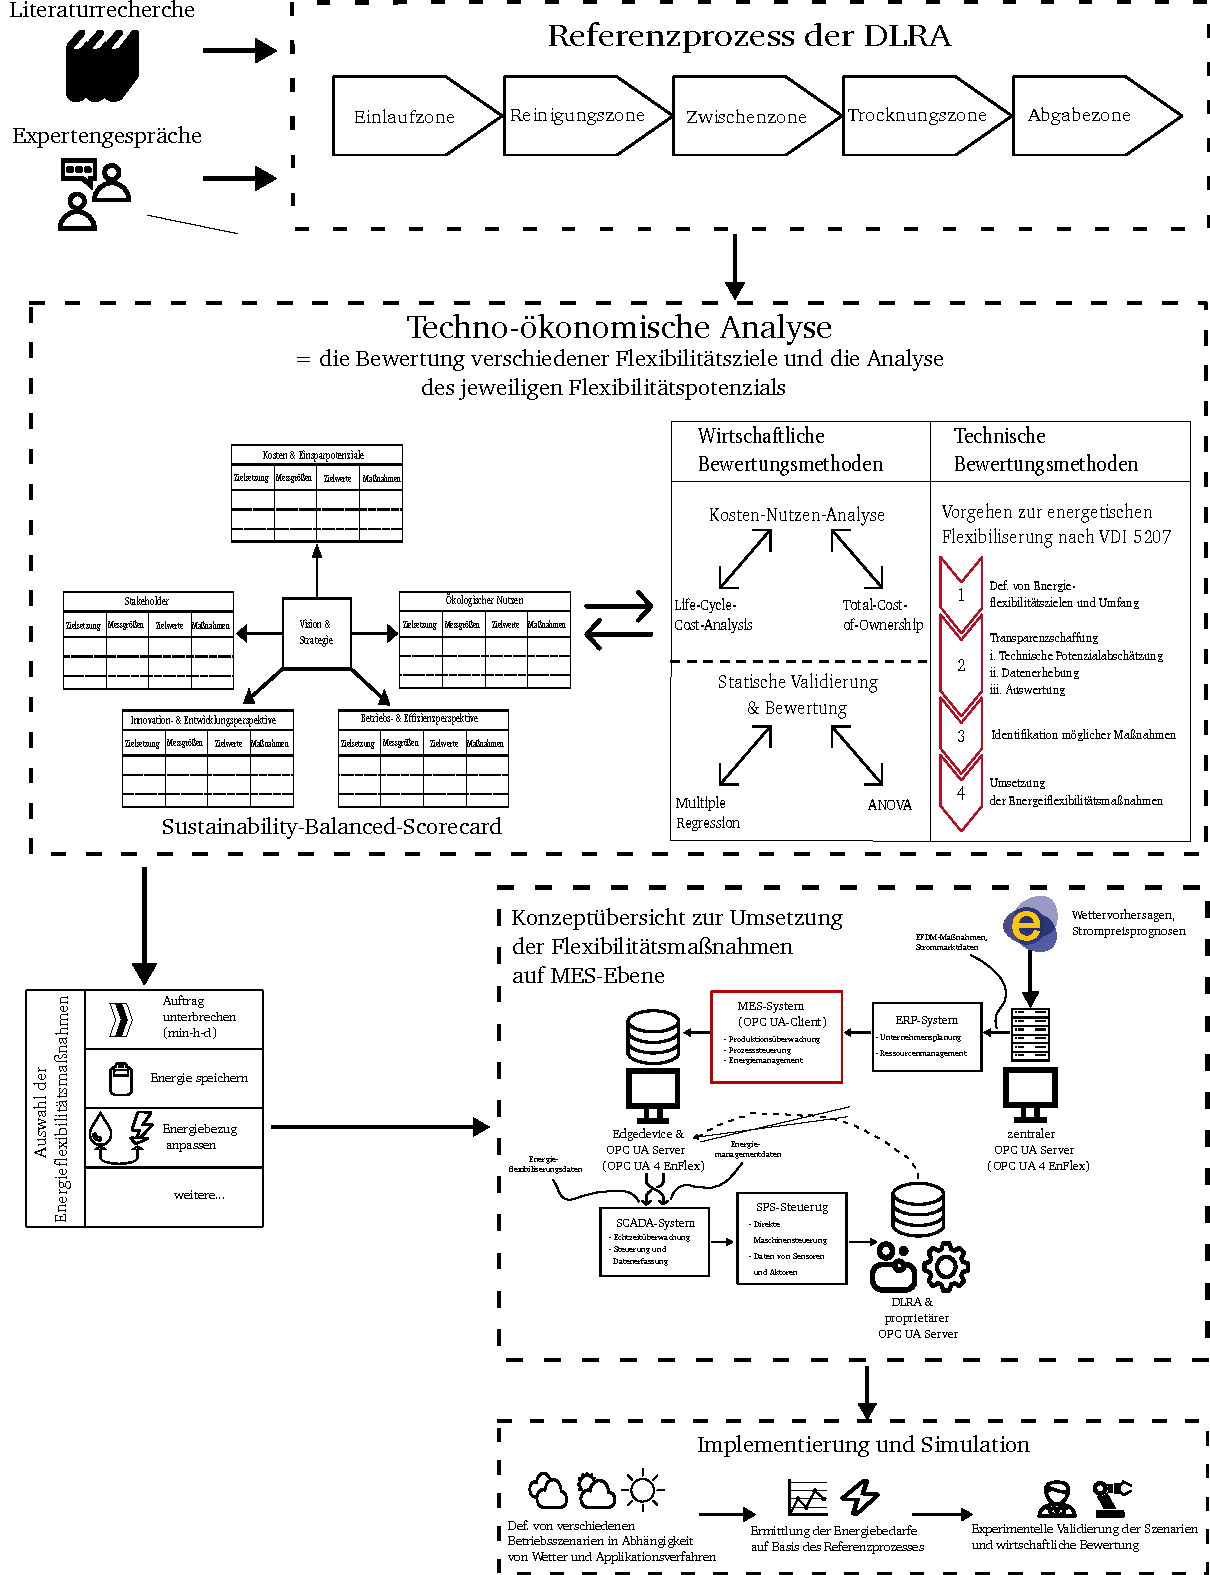
\includegraphics[width=\textwidth]{C:/Users/Anwender/Desktop/LaTeX_Template_Abschlussarbeit_TexStudio/figures/04_Aktueller Forschungsstand und Forschungsfrage/BigPicture.pdf}
	\caption{Beschreibung des Bildes}
	\label{fig_BigPicture}
\end{figure}


\section{Durchlaufreinigungsanlage (DLRA)}
\label{ch_04Durchlaufreinigungsanlage (DLRA)}
Weiteres bla bla bla...

\subsection{Beschreibung des praktischen Anwendungsfalls}
\label{ch_04Beschreibung des praktischen Anwendungsfalls}
Text

\subsection{Bedeutung für die Energieflexibilisierung}
\label{ch_04Bedeutung für die Energieflexibilisierung}
Text
\section{ETA-Fabrik}
\label{ch_04ETA-Fabrik}

\begin{itemize}
	\item Überblick über die ETA-Fabrik und deren Relevanz für die Studie
\end{itemize}
\section{SynErgie-Projekt}
\label{ch_04SynErgie-Projekt}
\begin{itemize}
	\item Beschreibung des Projektes und dessen Beitrag zur Energieflexibilisierung
\end{itemize}
\section{Ansteuerung von Datenpunkten mittels OPC-UA-Schnittstelle}
\label{ch_04Ansteuerung von Datenpunkten mittels OPC-UA-Schnittstelle}
\begin{itemize}
	\item Technische Details und Implementierung
\end{itemize}
\input{texts/04_Aktueller Forschungsstand und Forschungsfrage/Implementierung von Energieflexibilitätsmaßnahmen auf Fertigungsebene.tex}
\section{Forschungsziel und Fragen}
\label{ch_04Forschungsziel und Fragen}

Das Ziel der Masterthesis besteht darin, ein Konzept zur Implementierung geeigneter Flexibilitätsmaßnahmen auf der MES-Ebene für die DLRA zu entwickeln und anhand verschiedener Betriebsszenarien den zugehörigen Energiebedarf auf Basis des Referenzprozesses zu ermitteln. Nach der experimentellen Validierung der Szenarien soll eine wirtschaftliche Bewertung der implementierten Maßnahmen erfolgen.

Im Rahmen dieser Arbeit sollen folgende Forschungsfragen untersucht werden:

\begin{enumerate}[label=\textbf{\arabic*.}]
	\item \textbf{Kosteneffizienz der Energieflexibilitätsmaßnahmen:}\\ \emph{In welchem Umfang übersteigen die Einsparungen durch die Implementierung von Energieflexibilitätsmaßnahmen die damit verbundenen Kosten, und welche spezifischen Kostenfaktoren beeinflussen diese Bilanz?}
	
	Es ist entscheidend, zwischen den fixen Kosten, die durch die Implementierung der Maßnahmen entstehen, und der fortlaufenden Reduktion der variablen Betriebskosten der entsprechenden Anlage zu differenzieren. Diese Unterscheidung ermöglicht eine präzisere Bewertung der Kosteneffizienz. Ein zentrales Element ist die Berechnung der Amortisationszeit der Investition, um den Zeitraum zu bestimmen, in dem die Maßnahme wirtschaftlich wird. Darüber hinaus muss die Skalierbarkeit der Lösung über die OPC UA Schnittstelle berücksichtigt werden, da dies die Übertragung der Vorteile auf andere Anlagen erleichtert und somit eine breitere Anwendung ermöglicht.
	
	Ein weiterer wichtiger Aspekt im Zusammenhang mit dieser Forschungsfrage ist die Übertragbarkeit der in dieser Arbeit entwickelten und getesteten Flexibilitätsmaßnahmen auf industrielle Anwendungen. Es müssen spezifische Anpassungen ermittelt werden, um die Maßnahmen in einem realen industriellen Umfeld erfolgreich umzusetzen. Dies umfasst die Berücksichtigung der technischen Anforderungen sowie die Anpassung an unterschiedliche Betriebsbedingungen und Produktionsprozesse. Eine erfolgreiche Übertragung der Maßnahmen kann die wirtschaftlichen Vorteile maximieren und zu einer breiteren Akzeptanz und Anwendung in der Industrie führen.
	
	\item \textbf{Einflussfaktoren auf den Energiebedarf:}\\\emph{Welche spezifischen Einflussfaktoren aus Wetterdaten und Lastprofilen beeinflussen in welchem Ausmaß den Energiebedarf unter verschiedenen Betriebsszenarien und -strategien der Durchlaufreinigungsanlage (DLRA), und wie wirkt sich die Volatilität des Wetters in Kombination mit unterschiedlichen Lastprofilen auf die Umsetzung der Energieflexibilitätsmaßnahmen} aus?
	
	In Kapitel \ref{ch_05Ausarbeitung eines geeigneten Referenzprozesses} wird neben der Ausarbeitung eines geeigneten Referenzprozesses, auch verschiedene Marktszenarien definiert. Aus der Kombination dieser Marktszenarien und des Referenzprozesses werden die Betriebsszenarien hergeleitet, die für die Analyse und Beantwortung der Forschungsfrage verwendet werden. 
	
\end{enumerate}

Durch die Beantwortung dieser Fragen wird ein umfassendes Verständnis darüber gewonnen, wie eine energetische Flexibilisierung des Betriebs einer DLRA unter Berücksichtigung technischer und ökonomischer Faktoren optimiert werden kann.\\

Auf Grundlage der Forschungsfragen und spezifischer Aspekte der Untersuchung werden weitere Untersuchungshypothesen aufgestellt. Einige der Hypothesen sind auf Prädiktoren zurückzuführen, welche im Rahmen der multiplen Regression und einer ANOVA untersucht werden.\\

\textbf{Einfluss von spezifischen technischen Maßnahmen auf den Energieverbrauch:}

\begin{itemize}[label={--}]
	\item \textbf{\textit{$H_0$:}} \textit{Die Implementierung einer spezifischen Flexibilitätsmaßnahme (z.B. Nutzung der Speicherkapazität der Spültanks) führt nicht zu einer signifikanten Reduktion des Energieverbrauchs.}
	\item \textbf{\textit{$H_1$:}} \textit{Die Implementierung einer spezifischen Flexibilitätsmaßnahme (z.B. Nutzung der Speicherkapazität der Spültanks) führt zu einer signifikanten Reduktion des Energieverbrauchs.}\\
	\begin{itemize}
		\item \textbf{Durchlaufgeschwindigkeit:}
		\begin{itemize}
			\item \textbf{\textit{$H_0$:}} \textit{Eine Anpassung der Durchlaufgeschwindigkeit hat keinen signifikanten Einfluss auf den Energiebedarf.}
			\item \textbf{\textit{$H_1$:}} \textit{Eine Anpassung der Durchlaufgeschwindigkeit hat einen signifikanten Einfluss auf den Energiebedarf.}\\
		\end{itemize}
		\item \textbf{Reinigungstemperatur:}
		\begin{itemize}
			\item \textbf{\textit{$H_0$:}} \textit{Eine Anpassung der Reinigungstemperatur hat keinen signifikanten Einfluss auf den Energiebedarf.}
			\item \textbf{\textit{$H_1$:}} \textit{Eine Anpassung der Reinigungstemperatur hat einen signifikanten Einfluss auf den Energiebedarf.}\\\\
		\end{itemize}
	\end{itemize}
\end{itemize}

\textbf{Interaktionseffekte zwischen verschiedenen Einflussfaktoren:}
\begin{itemize}[label={--}]
	\item \textbf{\textit{$H_0$:}} \textit{Es gibt keine signifikanten Interaktionseffekte zwischen Wetterdaten und Lastprofilen auf den Energiebedarf.}
	\item \textbf{\textit{$H_1$:}} \textit{Es gibt signifikante Interaktionseffekte zwischen Wetterdaten und Lastprofilen auf den Energiebedarf.}\\\\
\end{itemize}

\textbf{Hypothesen zur Forschungsfrage 1:}
\begin{itemize}[label={--}]
	\item \textbf{\textit{$H_0$:}} \textit{Die Einsparungen durch die Implementierung von Energieflexibilitätsmaßnahmen übersteigen nicht die damit verbundenen Kosten.}
	\item \textbf{\textit{$H_1$:}} \textit{Die Einsparungen durch die Implementierung von Energieflexibilitätsmaßnahmen übersteigen die damit verbundenen Kosten.}
\end{itemize}

Beide Hypothesen bauen auf der ersten Forschungsfrage auf, wobei die erste Hypothese den Kostenfaktor und die zweite Hypothese die industrielle Anwendbarkeit untersucht.

\begin{itemize}[label={--}]
	\item \textbf{\textit{$H_0$:}} \textit{Die im Rahmen der Arbeit entwickelten Flexibilitätsmaßnahmen sind nicht auf industrielle Anwendungen übertragbar.}
	\item \textbf{\textit{$H_1$:}} \textit{Die im Rahmen der Arbeit entwickelten Flexibilitätsmaßnahmen sind auf industrielle Anwendungen übertragbar.}\\
	\begin{itemize}
		\item \textbf{Anpassungskosten:}
		\begin{itemize}
			\item \textbf{\textit{$H_0$:}} \textit{Die Kosten für die Anpassung der Maßnahmen an industrielle Anwendungen sind zu hoch, um eine Übertragbarkeit zu ermöglichen.}
			\item \textbf{\textit{$H_1$:}} \textit{Die Kosten für die Anpassung der Maßnahmen an industrielle Anwendungen sind nicht zu hoch, um eine Übertragbarkeit zu ermöglichen.}
		\end{itemize}
		\item \textbf{Technische Anpassungsfähigkeit:}
		\begin{itemize}
			\item \textbf{\textit{$H_0$:}} \textit{Die technischen Anpassungen, die für die Übertragbarkeit erforderlich sind, sind nicht durchführbar.}
			\item \textbf{\textit{$H_1$:}} \textit{Die technischen Anpassungen, die für die Übertragbarkeit erforderlich sind, sind durchführbar.}\\\\
		\end{itemize}
	\end{itemize}
\end{itemize}

\textbf{Hypothesen zur Forschungsfrage 2:}
\begin{itemize}[label={--}]
	\item \textbf{\textit{$H_0$:}} \textit{Wetterdaten und Lastprofile haben keinen signifikanten Einfluss auf den Energiebedarf der DLRA.}
	\item \textbf{\textit{$H_1$:}} \textit{Wetterdaten und Lastprofile haben einen signifikanten Einfluss auf den Energiebedarf der DLRA.}\\
	\begin{itemize}
		\item \textbf{Temperatur:} 
		\begin{itemize}
			\item \textbf{\textit{$H_0$:}} \textit{Die Temperatur hat keinen signifikanten Einfluss auf den Energiebedarf.}
			\item \textbf{\textit{$H_1$:}} \textit{Die Temperatur hat einen signifikanten Einfluss auf den Energiebedarf.}
		\end{itemize}
		\item \textbf{Sonneneinstrahlung:}
		\begin{itemize}
			\item \textbf{\textit{$H_0$:}} \textit{Die Sonneneinstrahlung hat keinen signifikanten Einfluss auf den Energiebedarf.}
			\item \textbf{\textit{$H_1$:}} \textit{Die Sonneneinstrahlung hat einen signifikanten Einfluss auf den Energiebedarf.}
		\end{itemize}
		\item \textbf{Windgeschwindigkeit:}
		\begin{itemize}
			\item \textbf{\textit{$H_0$:}} \textit{Die Windgeschwindigkeit hat keinen signifikanten Einfluss auf den Energiebedarf.}
			\item \textbf{\textit{$H_1$:}} \textit{Die Windgeschwindigkeit hat einen signifikanten Einfluss auf den Energiebedarf.}\\
		\end{itemize}
	\end{itemize}
\end{itemize}

Die methodischen Ansätze zur Beantwortung der Forschungsfragen und Überprüfung der Hypothesen umfassen:

\begin{itemize}[label={--}]
	\item \textbf{Literaturrecherche:} Vertiefte Einarbeitung in die Themen Energieflexibilisierung, Strommarktdesign und wasserbasierte Teilereinigung.
	\item \textbf{Datenanalyse:} Import und Analyse von Wettervorhersagen und Strompreisprognosen aus Entso-E, um den Energiebedarf in Abhängigkeit von verschiedenen Szenarien zu modellieren.
	\item \textbf{Experimentelle Versuchsreihe:} Durchführung von Versuchen zur Validierung der Szenarien und Flexibilitätsmaßnahmen an einer realen DLRA in der ETA-Fabrik.
	\item \textbf{Wirtschaftliche Bewertung:} Analyse der Kosten und Einsparungen durch die implementierten Flexibilitätsmaßnahmen mittels verschiedener Modelle, um deren wirtschaftliche Rentabilität zu beurteilen.
	\item \textbf{Statistische Analysen:} Anwendung von multipler Regression und ANOVA, um die signifikanten Einflussfaktoren und Interaktionseffekte zu identifizieren.
\end{itemize}

Durch diese umfassenden methodischen Ansätze wird eine fundierte Grundlage für die Beantwortung der Forschungsfragen und die Validierung der aufgestellten Hypothesen geschaffen.





%%%%%%%%%%%%%%%%%%%%%%%%%%%%%%%%%%%%%%%%%%%%%%%%%%%%%%%%%%%%%%%%%%%%%%%%%%%%
% Optimierung
\chapter{Untersuchungsmethodik}
\label{ch_05Untersuchungsmethodik}

\section{Forschungsdesign}
\label{ch_05Forschungsdesign}


\subsection{Beschreibung des Forschungsansatzes}
\label{ch_05Beschreibung des Forschungsansatzes}
\begin{itemize}
	\item Qualitativ, quantitativ oder gemischte Methoden
\end{itemize}

\subsection{Begründung der Methodenauswahl}
\label{ch_05Begründung der Methodenauswahl}
\section{Datenerhebungsmethoden}
\label{ch_05Datenerhebungsmethoden}


\subsection{Beschreibung der verwendeten Methoden}
\label{ch_05Beschreibung der verwendeten Methoden}
\begin{itemize}
	\item z. B. Eneffco etc., Strompreisprognosen von Entso-E, Quellen und Tools zur Datengewinnung
\end{itemize}

\subsection{Stichprobenbeschreibung und -auswahl}
\label{ch_05Stichprobenbeschreibung und -auswahl}
\begin{itemize}
	\item so was wie welche Marktszenarien und Zeiträume betrachtet werden
\end{itemize}
\section{Datenanalyse}
\label{ch_05Datenanalyse}

\subsection{Vorgehensweise bei der Datenanalyse}
\label{ch_05Vorgehensweise bei der Datenanalyse}
\subsection{Verwendete Analysetools und -techniken}
\label{ch_05Verwendete Analysetools und -techniken}
\input{texts/05_Untersuchungsmethodik/Techno-ökonomische Auswahl und Bewertung von Flexibilitätszielen}
\section{Ausarbeitung eines geeigneten Referenzprozesses}
\label{ch_05Ausarbeitung eines geeigneten Referenzprozesses}
\begin{itemize}
	\item Methodik zur Erstellung des Referenzprozesses unter Einbeziehung von Expertenwissen
\end{itemize}


%%%%%%%%%%%%%%%%%%%%%%%%%%%%%%%%%%%%%%%%%%%%%%%%%%%%%%%%%%%%%%%%%%%%%%%%%%%%
% Verlgeich und Bewertung
\input{texts/06_Techno-ökonomische Analyse/06_Techno-ökonomische Analyse.tex}


%%%%%%%%%%%%%%%%%%%%%%%%%%%%%%%%%%%%%%%%%%%%%%%%%%%%%%%%%%%%%%%%%%%%%%%%%%%%
% Implementierung und Simulation
\input{texts/07_Implementierung und Simulation/07_Implementierung und Simulation.tex}

%%%%%%%%%%%%%%%%%%%%%%%%%%%%%%%%%%%%%%%%%%%%%%%%%%%%%%%%%%%%%%%%%%%%%%%%%%%%
% Ergebnisse 
\chapter{Ergebnisse}
\label{ch_08Ergebnisse}

\section{Darstellung der Ergebnisse}
\label{ch_08Darstellung der Ergebnisse}

\subsection{Präsentation der Ergebnisse der durchgeführten Energieflexibilitätsmaßnahmen}
\label{ch_08Präsentation der Ergebnisse der durchgeführten Energieflexibilitätsmaßnahmen}

\subsection{Vergleich der Soll- und Ist-Werte}
\label{ch_08Vergleich der Soll- und Ist-Werte}


\section{Diskussion der Ergebnisse}
\label{ch_08Diskussion der Ergebnisse}

\subsection{Interpretation der Ergebnisse im Kontext der Forschungsfragen}
\label{ch_08Interpretation der Ergebnisse im Kontext der Forschungsfragen}

\subsection{Vergleich mit bisherigen Forschungsergebnissen}
\label{ch_08Vergleich mit bisherigen Forschungsergebnissen}


%%%%%%%%%%%%%%%%%%%%%%%%%%%%%%%%%%%%%%%%%%%%%%%%%%%%%%%%%%%%%%%%%%%%%%%%%%%%
% Diskussion und Schlussfolgerung
\input{texts/09_Diskussion und Schlussfolgerung/09_Diskussion und Schlussfolgerung.tex}
%%%%%%%%%%%%%%%%%%%%%%%%%%%%%%%%%%%%%%%%%%%%%%%%%%%%%%%%%%%%%%%%%%%%%%%%%%%%
% Umstellung auf römische Zahlen (es wird beim gespeicherten Wert weiter gezählt)
\newpage
\pagenumbering{Roman}
\setcounter{page}{\value{savecounter}}
%\backmatter

%%%%%%%%%%%%%%%%%%%%%%%%%%%%%%%%%%%%%%%%%%%%%%%%%%%%%%%%%%%%%%%%%%%%%%%%%%%%
% Anhang
\begin{appendix}
\chapter{Anhang}
\label{ch_99Anhang}
%\section{Berechnung der Koeffizienten für die dimensionslose Luftspaltleitwertfunktion}
%\label{ch_99FunktionLeit}
%In \cite{Kolbe.1983} empirisch ermittelte Gewichtsfunktion
%%
%\begin{equation}
%\label{equ_99FunktionLeit1}
%a_\lambda =
%\begin{cases}
%     e^{-\frac{1}{6}\left(\frac{b_\textsf{Q}}{\delta} - 1 \right)}, & \text{für} \quad \frac{b_\textsf{Q}}{\delta}\geq 10.6\\
%    \sin^4\left(\frac{\pi}{2} \frac{19- \frac{b_\textsf{Q}}{\delta}}{18} \right),              & \text{für} \quad \frac{b_\textsf{Q}}{\delta} < 10.6
%\end{cases}
%\end{equation}
%%
%und
%%
%\begin{equation}
%\label{equ_99FunktionLeit2}
%b_\lambda = 1 - a_\lambda.
%\end{equation}
%%
%Größe
%%
%\begin{equation}
%\label{equ_99FunktionLeit3}
%\beta_\lambda = 0.5 - \left[4 + \left(\frac{b_\textsf{Q}}{\delta} \right)^2 \right]^{-0.5}
%\end{equation}
%%
%nach Carter für die Ermittlung der Tiefe des Feldeinbruchs in der Nutmitte \cite{Carter.1901}.
%
%Empirisch in \cite{Kolbe.1983} bestimmte äquivalente Nutschlitzbreite:
%%
%\begin{equation}
%\label{equ_99FunktionLeit4}
%b_\textsf{0} = b_\textsf{Q} \left[ 1 + \left(0.8 + 10^{-4}\left(\frac{b_\textsf{Q}}{\delta} - 6\right)^4 \right) \cdot e^{-\frac{1}{8.5}\left(\frac{b_\textsf{Q}}{\delta} - 0.9 \right)} \right]
%\end{equation}
%%
%Die für die Funktion des dimensionslosen Luftspaltleitwerts benötigten Koeffizienten
%%
%\begin{equation}
%\label{equ_99FunktionLeit5}
%\tilde{\lambda}_\textsf{0} = 2 \left[1-\beta_\lambda \frac{b_\textsf{0}}{\tau_\textsf{Q}}\left(a_\lambda + b_\lambda \frac{11}{8} \right) \right]
%\end{equation}
%%
%und
%%
%\begin{equation}
%\label{equ_99FunktionLeit6}
%\tilde{\lambda}_{\nu_\textsf{S}} = \frac{\beta_\lambda}{\pi \nu_\textsf{S}} \sin\left(\frac{\pi}{x_{\nu_\textsf{S}}} \right) \left[\frac{2 a_\lambda}{\frac{1}{x_{\nu_\textsf{S}}^2}-1} + \frac{b_\lambda}{8} \left( \frac{15}{1- x_{\nu_\textsf{S}}^2} + \frac{6}{1- 4x_{\nu_\textsf{S}}^2} + \frac{1}{1- 9x_{\nu_\textsf{S}}^2} -22 \right) \right]
%\end{equation}
%%
%können zusammen mit der Hilfsgröße
%%
%\begin{equation}
%\label{equ_99FunktionLeit7}
%x_{\nu_\textsf{S}} = \frac{1}{\nu_\textsf{S} \frac{b_\textsf{0}}{\tau_\textsf{Q}}}
%\end{equation}
%%
%berechnet werden \cite{Kolbe.1983}.
%
%\newpage
%\section{Berechnung der dimensionslosen Geometrieeinfluss-Koeffizienten}
%\label{ch_99FunktionAnaly}
%Nachfolgend die Berechnung der dimensionslosen Geometrieeinfluss-Koeffizienten $\rho_\textsf{1,\nu}$ bis $\rho_\textsf{4,\nu}$ nach \cite{Barcaro.2011}:
%%
%\begin{equation}
%\begin{aligned}
%\rho_{\textsf{1,}\nu} = &(a+z(b-c+y(d-e+x(g-h))))\sin\left(\nu p \vartheta_\textsf{fb,1}\right) \\
% &+ z(c+y(e-f+x(h-k)))\sin\left(\nu p \vartheta_\textsf{fb,2}\right) \\
% &+ z\cdot y(f+x(k-l))\sin\left(\nu p \vartheta_\textsf{fb,3}\right) \\
% &+ z\cdot y\cdot x\cdot l\cdot \sin\left(\nu p \vartheta_\textsf{fb,4}\right)
%\end{aligned}
%\label{equ_99FunktionAnaly1}
%\end{equation}
%%
%%
%\begin{equation}
%\begin{aligned}
%\rho_{\textsf{2,}\nu} = &(b-c+y(d-e+x(g-h)))\sin\left(\nu p \vartheta_\textsf{fb,1}\right) \\
% &+ (c+y(e-f+x(h-k)))\sin\left(\nu p \vartheta_\textsf{fb,2}\right) \\
% &+ y(f+x(k-l))\sin\left(\nu p \vartheta_\textsf{fb,3}\right) \\
% &+ y\cdot x\cdot l\cdot \sin\left(\nu p \vartheta_\textsf{fb,4}\right)
%\end{aligned}
%\label{equ_99FunktionAnaly2}
%\end{equation}
%%
%%
%\begin{equation}
%\begin{aligned}
%\rho_{\textsf{3,}\nu} = &(d-e+x(g-h))\sin\left(\nu p \vartheta_\textsf{fb,1}\right) \\
% &+ (e-f+x(h-k))\sin\left(\nu p \vartheta_\textsf{fb,2}\right) \\
% &+ (f+x(k-l))\sin\left(\nu p \vartheta_\textsf{fb,3}\right) \\
% &+ x\cdot l\cdot \sin\left(\nu p \vartheta_\textsf{fb,4}\right)
%\end{aligned}
%\label{equ_99FunktionAnaly3}
%\end{equation}
%%
%%
%\begin{equation}
%\begin{aligned}
%\rho_{\textsf{4,}\nu} = &(g-h)\sin\left(\nu p \vartheta_\textsf{fb,1}\right) \\
% &+ (h-k)\sin\left(\nu p \vartheta_\textsf{fb,2}\right) \\
% &+ (k-l)\sin\left(\nu p \vartheta_\textsf{fb,3}\right) \\
% &+ l\cdot \sin\left(\nu p \vartheta_\textsf{fb,4}\right)
%\end{aligned}
%\label{equ_99FunktionAnaly4}
%\end{equation}
%%
%%
%\begin{equation}
%a = \left(\frac{d_\textsf{Si}}{2\delta} \frac{w_\textsf{fb,1}}{l_\textsf{fb,1}}\right) \cdot z
%\label{equ_99FunktionAnaly5}
%\end{equation}
%%
%%
%\begin{equation}
%z = \frac{1}{1 + \frac{d_\textsf{Si}}{\delta} \frac{w_\textsf{fb,1}}{l_\textsf{fb,1}} \vartheta_\textsf{fb,1}}
%\label{equ_99FunktionAnaly6}
%\end{equation}
%%
%%
%\begin{equation}
%b = \left(a \frac{l_\textsf{fb,1}}{w_\textsf{fb,1}} \frac{w_\textsf{fb,2}}{l_\textsf{fb,2}}\right) \cdot y
%\label{equ_99FunktionAnaly7}
%\end{equation}
%%
%%
%\begin{equation}
%c = \left(\frac{d_\textsf{Si}}{2\delta} \frac{w_\textsf{fb,2}}{l_\textsf{fb,2}}\right) \cdot y
%\label{equ_99FunktionAnaly8}
%\end{equation}
%%
%%
%\begin{equation}
%y = \frac{1}{1 - (z-1)\frac{l_\textsf{fb,1}}{w_\textsf{fb,1}} \frac{w_\textsf{fb,2}}{l_\textsf{fb,2}} + \frac{d_\textsf{Si}}{\delta} \frac{w_\textsf{fb,2}}{l_\textsf{fb,2}} \left(\vartheta_\textsf{fb,2} - \vartheta_\textsf{fb,1}\right)}
%\label{equ_99FunktionAnaly9}
%\end{equation}
%%
%%
%\begin{equation}
%d = \left(b \frac{l_\textsf{fb,2}}{w_\textsf{fb,2}} \frac{w_\textsf{fb,3}}{l_\textsf{fb,3}}\right) \cdot x
%\label{equ_99FunktionAnaly10}
%\end{equation}
%%
%%
%\begin{equation}
%e = \left(c \frac{l_\textsf{fb,2}}{w_\textsf{fb,2}} \frac{w_\textsf{fb,3}}{l_\textsf{fb,3}}\right) \cdot x
%\label{equ_99FunktionAnaly11}
%\end{equation}
%%
%%
%\begin{equation}
%f = \left(\frac{d_\textsf{Si}}{2\delta} \frac{w_\textsf{fb,3}}{l_\textsf{fb,3}}\right) \cdot x
%\label{equ_99FunktionAnaly12}
%\end{equation}
%%
%%
%\begin{equation}
%x = \frac{1}{1 - (y-1)\frac{l_\textsf{fb,2}}{w_\textsf{fb,2}} \frac{w_\textsf{fb,3}}{l_\textsf{fb,3}} + \frac{d_\textsf{Si}}{\delta} \frac{w_\textsf{fb,3}}{l_\textsf{fb,3}} \left(\vartheta_\textsf{fb,3} - \vartheta_\textsf{fb,2}\right)}
%\label{equ_99FunktionAnaly13}
%\end{equation}
%%
%%
%\begin{equation}
%g = \left(d \frac{l_\textsf{fb,3}}{w_\textsf{fb,3}} \frac{w_\textsf{fb,4}}{l_\textsf{fb,4}}\right) \cdot w
%\label{equ_99FunktionAnaly14}
%\end{equation}
%%
%%
%\begin{equation}
%h = \left(e \frac{l_\textsf{fb,3}}{w_\textsf{fb,3}} \frac{w_\textsf{fb,4}}{l_\textsf{fb,4}}\right) \cdot w
%\label{equ_99FunktionAnaly15}
%\end{equation}
%%
%%
%\begin{equation}
%k = \left(f \frac{l_\textsf{fb,3}}{w_\textsf{fb,3}} \frac{w_\textsf{fb,4}}{l_\textsf{fb,4}}\right) \cdot w
%\label{equ_99FunktionAnaly16}
%\end{equation}
%%
%%
%\begin{equation}
%l = \left(\frac{d_\textsf{Si}}{2\delta} \frac{w_\textsf{fb,4}}{l_\textsf{fb,4}}\right) \cdot w
%\label{equ_99FunktionAnaly17}
%\end{equation}
%%
%%
%\begin{equation}
%w = \frac{1}{1 - (x-1)\frac{l_\textsf{fb,3}}{w_\textsf{fb,3}} \frac{w_\textsf{fb,4}}{l_\textsf{fb,4}} + \frac{d_\textsf{Si}}{\delta} \frac{w_\textsf{fb,4}}{l_\textsf{fb,4}} \left(\vartheta_\textsf{fb,4} - \vartheta_\textsf{fb,3}\right)}
%\label{equ_99FunktionAnaly18}
%\end{equation}
%%
%An dieser stelle sei angemerkt, dass die Notation hier von der in \cite{Barcaro.2011} abweicht.
%
%\section{Ergebnisse des Berechnungsskripts und der FE-gestützten Optimierung}
%\label{ch_99MagSimErg}
%
%\begin{figure}[H]
%\centering
%\def\svgwidth{490pt}
%\input{figures/99_Anhang/rel_rippel_sym.pdf_tex}
%\caption[Relative Drehmomentwelligkeit der Variante 1 über den Flusssperrenpositionen]{Relative Drehmomentwelligkeit der getesteten Rotorgeometrien der Variante 1 aufgetragen über den Flusssperrenpositionen: links Berechnungsskript, rechts FE-Simulation}
%\label{fig_99MagSimErg1}
%\end{figure}
%\quad
\end{appendix}


%%%%%%%%%%%%%%%%%%%%%%%%%%%%%%%%%%%%%%%%%%%%%%%%%%%%%%%%%%%%%%%%%%%%%%%%%%%%
% Literaturverzeichnis
\newpage
\addcontentsline{toc}{chapter}{Literaturverzeichnis}
\renewcommand{\bibname}{Literaturverzeichnis} 	% Umbenennung des Literaturverzeichnisses 
\printbibliography
\phantomsection


\end{document}